\hypertarget{functions-in-tfetextview}{%
\section{Functions in TfeTextView}\label{functions-in-tfetextview}}

In this section I will explain functions in TfeTextView object.

\hypertarget{tfe.h-and-tfetextview.h}{%
\subsection{tfe.h and tfetextview.h}\label{tfe.h-and-tfetextview.h}}

\passthrough{\lstinline!tfe.h!} is a top header file and it includes
\passthrough{\lstinline!gtk.h!} and all the header files. C source files
\passthrough{\lstinline!tfeapplication.c!} and
\passthrough{\lstinline!tfenotebook.c!} include
\passthrough{\lstinline!tfe.h!} at the beginning.

\begin{lstlisting}[language=C, numbers=left]
#include <gtk/gtk.h>

#include "../tfetextview/tfetextview.h"
#include "tfenotebook.h"
\end{lstlisting}

\passthrough{\lstinline!../tfetextview/tfetextview.h!} is a header file
which describes the public functions in
\passthrough{\lstinline!tfetextview.c!}.

\begin{lstlisting}[language=C, numbers=left]
#ifndef __TFE_TEXT_VIEW_H__
#define __TFE_TEXT_VIEW_H__

#include <gtk/gtk.h>

#define TFE_TYPE_TEXT_VIEW tfe_text_view_get_type ()
G_DECLARE_FINAL_TYPE (TfeTextView, tfe_text_view, TFE, TEXT_VIEW, GtkTextView)

/* "open-response" signal response */
enum TfeTextViewOpenResponseType
{
  TFE_OPEN_RESPONSE_SUCCESS,
  TFE_OPEN_RESPONSE_CANCEL,
  TFE_OPEN_RESPONSE_ERROR
};

GFile *
tfe_text_view_get_file (TfeTextView *tv);

void
tfe_text_view_open (TfeTextView *tv, GtkWindow *win);

void
tfe_text_view_save (TfeTextView *tv);

void
tfe_text_view_saveas (TfeTextView *tv);

GtkWidget *
tfe_text_view_new_with_file (GFile *file);

GtkWidget *
tfe_text_view_new (void);

#endif /* __TFE_TEXT_VIEW_H__ */
\end{lstlisting}

\begin{itemize}
\tightlist
\item
  1,2,35: Thanks to these three lines, the following lines are included
  only once.
\item
  4: Includes gtk4 header files. The header file
  \passthrough{\lstinline!gtk4!} also has the same mechanism to avoid
  including it multiple times.
\item
  6-7: These two lines define TfeTextView type, its class structure and
  some useful macros.
\item
  9-15: A definition of the value of the parameter of ``open-response''
  signal.
\item
  17-33: Declarations of public functions on TfeTextView.
\end{itemize}

\hypertarget{functions-to-create-tfetextview-instances}{%
\subsection{Functions to create TfeTextView
instances}\label{functions-to-create-tfetextview-instances}}

A TfeTextView instance is created with
\passthrough{\lstinline!tfe\_text\_view\_new!} or
\passthrough{\lstinline!tfe\_text\_view\_new\_with\_file!}.

\begin{lstlisting}[language=C]
GtkWidget *tfe_text_view_new (void);
\end{lstlisting}

\passthrough{\lstinline!tfe\_text\_view\_new!} just creates a new
TfeTextView instance and returns the pointer to the new instance.

\begin{lstlisting}[language=C]
GtkWidget *tfe_text_view_new_with_file (GFile *file);
\end{lstlisting}

\passthrough{\lstinline!tfe\_text\_view\_new\_with\_file!} is given a
Gfile object as an argument and it loads the file into the GtkTextBuffer
instance, then returns the pointer to the new instance. If an error
occurs during the creation process, NULL is returned.

Each function is defined as follows.

\begin{lstlisting}[language=C, numbers=left]
GtkWidget *
tfe_text_view_new_with_file (GFile *file) {
  g_return_val_if_fail (G_IS_FILE (file), NULL);

  GtkWidget *tv;
  GtkTextBuffer *tb;
  char *contents;
  gsize length;

  if (! g_file_load_contents (file, NULL, &contents, &length, NULL, NULL)) /* read error */
    return NULL;

  if ((tv = tfe_text_view_new()) != NULL) {
    tb = gtk_text_view_get_buffer (GTK_TEXT_VIEW (tv));
    gtk_text_buffer_set_text (tb, contents, length);
    TFE_TEXT_VIEW (tv)->file = g_file_dup (file);
    gtk_text_buffer_set_modified (tb, FALSE);
  }
  g_free (contents);
  return tv;
}

GtkWidget *
tfe_text_view_new (void) {
  return GTK_WIDGET (g_object_new (TFE_TYPE_TEXT_VIEW, NULL));
}
\end{lstlisting}

\begin{itemize}
\tightlist
\item
  23-25: \passthrough{\lstinline!tfe\_text\_view\_new!} function. Just
  returns the value from the function
  \passthrough{\lstinline!g\_object\_new!} but casts it to the pointer
  to GtkWidget. Initialization is done in
  \passthrough{\lstinline!tfe\_text\_view\_init!} which is called in the
  process of \passthrough{\lstinline!g\_object\_new!} function.
\item
  1-21: \passthrough{\lstinline!tfe\_text\_view\_new\_with\_file!}
  function.
\item
  3: \passthrough{\lstinline!g\_return\_val\_if\_fail!} is described in
  \href{https://docs.gtk.org/glib/func.return_val_if_fail.html}{GLib API
  Reference, g\_return\_val\_if\_fail}. And also
  \href{https://docs.gtk.org/glib/logging.html}{GLib API Reference,
  Message Logging}. It tests whether the argument
  \passthrough{\lstinline!file!} is a pointer to GFile. If it's true,
  then the program goes on to the next line. If it's false, then it
  returns NULL (the second argument) immediately. And at the same time
  it logs out the error message (usually the log is outputted to stderr
  or stdout). This function is used to check the programmer's error. If
  an error occurs, the solution is usually to change the (caller)
  program and fix the bug. You need to distinguish programmer's errors
  and runtime errors. You shouldn't use this function to find runtime
  errors.
\item
  10-11: If an error occurs when reading the file, then the function
  returns NULL.
\item
  13: Calls the function \passthrough{\lstinline!tfe\_text\_view\_new!}.
  The function creates TfeTextView instance and returns the pointer to
  the instance. If an error happens in
  \passthrough{\lstinline!tfe\_text\_view\_new!}, it returns NULL.
\item
  14: Gets the pointer to GtkTextBuffer corresponds to
  \passthrough{\lstinline!tv!}. The pointer is assigned to
  \passthrough{\lstinline!tb!}
\item
  15: Assigns the contents read from the file to GtkTextBuffer pointed
  by \passthrough{\lstinline!tb!}.
\item
  16: Duplicates \passthrough{\lstinline!file!} and sets
  \passthrough{\lstinline!tv->file!} to point it.
\item
  17: The function
  \passthrough{\lstinline!gtk\_text\_buffer\_set\_modified (tb, FALSE)!}
  sets the modification flag of \passthrough{\lstinline!tb!} to FALSE.
  The modification flag indicates that the contents of the buffer is
  modified. It is used when the contents are saved. If the modification
  flag is FALSE, it doesn't need to save the contents.
\item
  19: Frees the memories pointed by \passthrough{\lstinline!contents!}.
\item
  20: Returns \passthrough{\lstinline!tv!}, which is a pointer to the
  newly created TfeTextView instance. If an error happens, NULL is
  returned.
\end{itemize}

\hypertarget{save-and-saveas-functions}{%
\subsection{Save and saveas functions}\label{save-and-saveas-functions}}

Save and saveas functions write the contents in the GtkTextBuffer to a
file.

\begin{lstlisting}[language=C]
void tfe_text_view_save (TfeTextView *tv)
\end{lstlisting}

The function \passthrough{\lstinline!tfe\_text\_view\_save!} writes the
contents in the GtkTextBuffer to a file specified by
\passthrough{\lstinline!tv->file!}. If
\passthrough{\lstinline!tv->file!} is NULL, then it shows
GtkFileChooserDialog and prompts the user to choose a file to save. Then
it saves the contents to the file and sets
\passthrough{\lstinline!tv->file!} to point the GFile instance for the
file.

\begin{lstlisting}[language=C]
void tfe_text_view_saveas (TfeTextView *tv)
\end{lstlisting}

The function \passthrough{\lstinline!saveas!} uses GtkFileChooserDialog
and prompts the user to select a existed file or specify a new file to
save. Then, the function changes \passthrough{\lstinline!tv->file!} and
save the contents to the specified file. If an error occurs, it is shown
to the user through the message dialog. The error is managed only in the
TfeTextView and no information is notified to the caller.

\begin{lstlisting}[language=C, numbers=left]
static gboolean
save_file (GFile *file, GtkTextBuffer *tb, GtkWindow *win) {
  GtkTextIter start_iter;
  GtkTextIter end_iter;
  gchar *contents;
  gboolean stat;
  GtkWidget *message_dialog;
  GError *err = NULL;

  gtk_text_buffer_get_bounds (tb, &start_iter, &end_iter);
  contents = gtk_text_buffer_get_text (tb, &start_iter, &end_iter, FALSE);
  if (g_file_replace_contents (file, contents, strlen (contents), NULL, TRUE, G_FILE_CREATE_NONE, NULL, NULL, &err)) {
    gtk_text_buffer_set_modified (tb, FALSE);
    stat = TRUE;
  } else {
    message_dialog = gtk_message_dialog_new (win, GTK_DIALOG_MODAL,
                                             GTK_MESSAGE_ERROR, GTK_BUTTONS_CLOSE,
                                            "%s.\n", err->message);
    g_signal_connect (message_dialog, "response", G_CALLBACK (gtk_window_destroy), NULL);
    gtk_widget_show (message_dialog);
    g_error_free (err);
    stat = FALSE;
  }
  g_free (contents);
  return stat;
}

static void
saveas_dialog_response (GtkWidget *dialog, gint response, TfeTextView *tv) {
  GtkTextBuffer *tb = gtk_text_view_get_buffer (GTK_TEXT_VIEW (tv));
  GFile *file;
  GtkWidget *win = gtk_widget_get_ancestor (GTK_WIDGET (tv), GTK_TYPE_WINDOW);

  if (response == GTK_RESPONSE_ACCEPT) {
    file = gtk_file_chooser_get_file (GTK_FILE_CHOOSER (dialog));
    if (! G_IS_FILE (file))
      g_warning ("TfeTextView: gtk_file_chooser_get_file returns non GFile.\n");
    else if (save_file(file, tb, GTK_WINDOW (win))) {
      if (G_IS_FILE (tv->file))
        g_object_unref (tv->file);
      tv->file = file;
      g_signal_emit (tv, tfe_text_view_signals[CHANGE_FILE], 0);
    } else
      g_object_unref (file);
  }
  gtk_window_destroy (GTK_WINDOW (dialog));
}

void
tfe_text_view_save (TfeTextView *tv) {
  g_return_if_fail (TFE_IS_TEXT_VIEW (tv));

  GtkTextBuffer *tb = gtk_text_view_get_buffer (GTK_TEXT_VIEW (tv));
  GtkWidget *win = gtk_widget_get_ancestor (GTK_WIDGET (tv), GTK_TYPE_WINDOW);

  if (! gtk_text_buffer_get_modified (tb))
    return; /* no need to save it */
  else if (tv->file == NULL)
    tfe_text_view_saveas (tv);
  else if (! G_IS_FILE (tv->file))
    g_error ("TfeTextView: The pointer tv->file isn't NULL nor GFile.\n");
  else
    save_file (tv->file, tb, GTK_WINDOW (win));
}

void
tfe_text_view_saveas (TfeTextView *tv) {
  g_return_if_fail (TFE_IS_TEXT_VIEW (tv));

  GtkWidget *dialog;
  GtkWidget *win = gtk_widget_get_ancestor (GTK_WIDGET (tv), GTK_TYPE_WINDOW);

  dialog = gtk_file_chooser_dialog_new ("Save file", GTK_WINDOW (win), GTK_FILE_CHOOSER_ACTION_SAVE,
                                      "Cancel", GTK_RESPONSE_CANCEL,
                                      "Save", GTK_RESPONSE_ACCEPT,
                                      NULL);
  g_signal_connect (dialog, "response", G_CALLBACK (saveas_dialog_response), tv);
  gtk_widget_show (dialog);
}
\end{lstlisting}

\begin{itemize}
\tightlist
\item
  1-26: \passthrough{\lstinline!save\_file!} function. This function is
  called from \passthrough{\lstinline!saveas\_dialog\_response!} and
  \passthrough{\lstinline!tfe\_text\_view\_save!}. This function saves
  the contents of the buffer to the file given as an argument. If error
  happens, it displays an error message. The class of this function is
  \passthrough{\lstinline!static!}. Therefore, only functions in this
  file (\passthrough{\lstinline!tfeTetview.c!}) call this function. Such
  static functions usally don't have
  \passthrough{\lstinline!g\_return\_val\_if\_fail!} function.
\item
  10-11: Gets the text contents from the buffer.
\item
  12-14: Saves the contents to the file. If no error happens, set the
  modified flag to be FALSE. This means that the buffer is not modified
  since it has been saved. And set the return status
  \passthrough{\lstinline!stat!} to be TRUE.
\item
  15-23: If it fails to save the contents, displays an error message.
\item
  16-18: Creates a message dialog with the error message.
\item
  19: Connects the ``response'' signal to
  \passthrough{\lstinline!gtk\_window\_destroy!}, so that the dialog
  disappears when a user clicked on the button.
\item
  20-21: Shows the window, frees \passthrough{\lstinline!err!} and set
  \passthrough{\lstinline!stat!} to be FLASE.
\item
  24: Frees \passthrough{\lstinline!contents!}.
\item
  25: Returns to the caller.
\item
  28-47: \passthrough{\lstinline!saveas\_dialog\_response!} function.
  This is a signal handler for the ``response'' signal on
  GtkFileChooserDialog instance created by
  \passthrough{\lstinline!tfe\_text\_view\_saveas!} function. This
  handler analyzes the response and determines whether to save the
  contents.
\item
  34-45: If the response is
  \passthrough{\lstinline!GTK\_RESPONSE\_ACCEPT!}, the user has clicked
  on the \passthrough{\lstinline!Save!} button. So, it tries to save.
\item
  35: Gets the GFile \passthrough{\lstinline!file!} from
  GtkFileChooserDialog.
\item
  36-37: If it doesn't point GFile, it outputs an error message to the
  log.
\item
  38: Otherwise, it calls \passthrough{\lstinline!save\_file!} to save
  the contents to the file.
\item
  39-42: If \passthrough{\lstinline!save\_file!} has successfully saved
  the contents, \passthrough{\lstinline!tv->file!} is updated. If the
  old GFile pointed by \passthrough{\lstinline!tv->file!} exists, it is
  freed in advance. Emits ``change-file'' signal.
\item
  44: Unrefs \passthrough{\lstinline!file!}.
\item
  46: destroys the file chooser dialog.
\item
  49-64: \passthrough{\lstinline!tfe\_text\_view\_save!} function.
\item
  51: \passthrough{\lstinline!tfe\_text\_view\_save!} is public, i.e.~it
  is open to the other files. So, it doesn't have
  \passthrough{\lstinline!static!} class. Public functions should check
  the parameter type with \passthrough{\lstinline!g\_return\_if\_fail!}
  function. If \passthrough{\lstinline!tv!} is not a pointer to a
  TfeTextView instance, then it logs an error message and immediately
  returns. This function is similar to
  \passthrough{\lstinline!g\_return\_val\_if\_fail!}, but no value is
  returned because \passthrough{\lstinline!tfe\_text\_view\_save!}
  doesn't return a value.
\item
  53-54: Gets GtkTextBuffer instance and GtkWidget instance and assignes
  them to \passthrough{\lstinline!tb!} and\passthrough{\lstinline!win!}
  respectively.
\item
  56-57: If the buffer hasn't modified, then it doesn't need to save it.
  So the function returns.
\item
  58-59: If \passthrough{\lstinline!tv->file!} is NULL, no file has
  given yet. It calls \passthrough{\lstinline!tfe\_text\_view\_saveas!}
  which prompts a user to select a file or specify a new file to save.
\item
  60-61: If \passthrough{\lstinline!tv->file!} doesn't point GFile,
  somethig bad has happened. Logs an error message.
\item
  62-63: Calls \passthrough{\lstinline!save\_file!} to save the contents
  to the file.
\item
  66-79: \passthrough{\lstinline!tfe\_text\_view\_saveas!} function. It
  shows GtkFileChooserDialog and prompts the user to choose a file.
\item
  73-76: Creates GtkFileChooserDialog. The title is ``Save file''.
  Transient parent of the dialog is \passthrough{\lstinline!win!}, which
  is the top-level window. The action is save mode. The buttons are
  Cancel and Save.
\item
  77: connects the ``response'' signal of the dialog and
  \passthrough{\lstinline!saveas\_dialog\_response!} handler.
\item
  78: Shows the dialog.
\end{itemize}

\begin{figure}
\centering
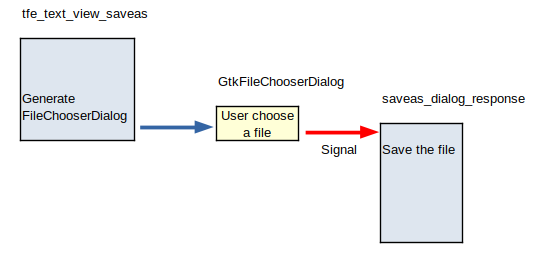
\includegraphics[width=10.7cm,height=5.16cm]{../image/saveas.png}
\caption{Saveas process}
\end{figure}

When you use GtkFileChooserDialog, you need to divide the program into
two parts. One is a function which creates GtkFileChooserDialog and the
other is a signal handler. The function just creates and shows
GtkFileChooserDialog. The rest is done by the handler. It gets Gfile
from GtkFileChooserDialog and saves the buffer to the file by calling
\passthrough{\lstinline!save\_file!}.

\hypertarget{open-function}{%
\subsection{Open function}\label{open-function}}

Open function shows GtkFileChooserDialog to users and prompts them to
choose a file. Then it reads the file and puts the text into
GtkTextBuffer.

\begin{lstlisting}[language=C]
void tfe_text_view_open (TfeTextView *tv, GtkWindow *win);
\end{lstlisting}

The parameter \passthrough{\lstinline!win!} is the top-level window. It
will be a transient parent window of GtkFileChooserDialog when the
dialog is created. This allows window managers to keep the dialog on top
of the parent window, or center the dialog over the parent window. It is
possible to give no parent window to the dialog. However, it is
encouraged to give a parent window to dialog. This function might be
called just after \passthrough{\lstinline!tv!} has been created. In that
case, \passthrough{\lstinline!tv!} has not been incorporated into the
widget hierarchy. Therefore it is impossible to get the top-level window
from \passthrough{\lstinline!tv!}. That's why the function needs
\passthrough{\lstinline!win!} parameter.

This function is usually called when the buffer of
\passthrough{\lstinline!tv!} is empty. However, even if the buffer is
not empty, \passthrough{\lstinline!tfe\_text\_view\_open!} doesn't treat
it as an error. If you want to revert the buffer, calling this function
is appropriate. Otherwise probably bad things will happen.

\begin{lstlisting}[language=C, numbers=left]
static void
open_dialog_response(GtkWidget *dialog, gint response, TfeTextView *tv) {
  GtkTextBuffer *tb = gtk_text_view_get_buffer (GTK_TEXT_VIEW (tv));
  GFile *file;
  char *contents;
  gsize length;
  GtkWidget *message_dialog;
  GError *err = NULL;

  if (response != GTK_RESPONSE_ACCEPT)
    g_signal_emit (tv, tfe_text_view_signals[OPEN_RESPONSE], 0, TFE_OPEN_RESPONSE_CANCEL);
  else if (! G_IS_FILE (file = gtk_file_chooser_get_file (GTK_FILE_CHOOSER (dialog)))) {
    g_warning ("TfeTextView: gtk_file_chooser_get_file returns non GFile.\n");
    g_signal_emit (tv, tfe_text_view_signals[OPEN_RESPONSE], 0, TFE_OPEN_RESPONSE_ERROR);
  } else if (! g_file_load_contents (file, NULL, &contents, &length, NULL, &err)) { /* read error */
    g_object_unref (file);
    message_dialog = gtk_message_dialog_new (GTK_WINDOW (dialog), GTK_DIALOG_MODAL,
                                             GTK_MESSAGE_ERROR, GTK_BUTTONS_CLOSE,
                                            "%s.\n", err->message);
    g_signal_connect (message_dialog, "response", G_CALLBACK (gtk_window_destroy), NULL);
    gtk_widget_show (message_dialog);
    g_error_free (err);
    g_signal_emit (tv, tfe_text_view_signals[OPEN_RESPONSE], 0, TFE_OPEN_RESPONSE_ERROR);
  } else {
    gtk_text_buffer_set_text (tb, contents, length);
    g_free (contents);
    if (G_IS_FILE (tv->file))
      g_object_unref (tv->file);
    tv->file = file;
    gtk_text_buffer_set_modified (tb, FALSE);
    g_signal_emit (tv, tfe_text_view_signals[OPEN_RESPONSE], 0, TFE_OPEN_RESPONSE_SUCCESS);
    g_signal_emit (tv, tfe_text_view_signals[CHANGE_FILE], 0);
  }
  gtk_window_destroy (GTK_WINDOW (dialog));
}

void
tfe_text_view_open (TfeTextView *tv, GtkWindow *win) {
  g_return_if_fail (TFE_IS_TEXT_VIEW (tv));
  g_return_if_fail (GTK_IS_WINDOW (win));

  GtkWidget *dialog;

  dialog = gtk_file_chooser_dialog_new ("Open file", win, GTK_FILE_CHOOSER_ACTION_OPEN,
                                        "Cancel", GTK_RESPONSE_CANCEL,
                                        "Open", GTK_RESPONSE_ACCEPT,
                                        NULL);
  g_signal_connect (dialog, "response", G_CALLBACK (open_dialog_response), tv);
  gtk_widget_show (dialog);
}
\end{lstlisting}

\begin{itemize}
\tightlist
\item
  37-50: \passthrough{\lstinline!tfe\_text\_view\_open!} function.
\item
  44-47: Creates GtkFileChooserDialog. The title is ``Open file''.
  Transient parent window is the top-level window of the application,
  which is given by the caller. The action is open mode. The buttons are
  Cancel and Open.
\item
  48: connects the ``response'' signal of the dialog and
  \passthrough{\lstinline!open\_dialog\_response!} signal handler.
\item
  49: Shows the dialog.
\item
  1-35: \passthrough{\lstinline!open\_dialog\_response!} signal handler.
\item
  10-11: If the response from GtkFileChooserDialog is not
  \passthrough{\lstinline!GTK\_RESPONSE\_ACCEPT!}, the user has clicked
  on the ``Cancel'' button or close button on the header bar. Then,
  ``open-response'' signal is emitted. The parameter of the signal is
  \passthrough{\lstinline!TFE\_OPEN\_RESPONSE\_CANCEL!}.
\item
  12-14: Gets the pointer to the Gfile by
  \passthrough{\lstinline!gtk\_file\_chooser\_get\_file!}. If it doesn't
  point GFile, maybe an error has occurred. Then it emits
  ``open-response'' signal with the parameter
  \passthrough{\lstinline!TFE\_OPEN\_RESPONSE\_ERROR!}.
\item
  15-23: If an error occurs at file reading, then it decreases the
  reference count of the Gfile, shows a message dialog to report the
  error to the user and emits ``open-response'' signal with the
  parameter \passthrough{\lstinline!TFE\_OPEN\_RESPONSE\_ERROR!}.
\item
  24-33: If the file has successfully been read, then the text is
  inserted to GtkTextBuffer, frees the temporary buffer pointed by
  \passthrough{\lstinline!contents!} and sets
  \passthrough{\lstinline!tv->file!} to point the file (no duplication
  is not necessary). Then, it emits ``open-response'' signal with the
  parameter \passthrough{\lstinline!TFE\_OPEN\_RESPONSE\_SUCCESS!} and
  emits ``change-file'' signal.
\item
  34: destroys GtkFileCooserDialog.
\end{itemize}

Now let's think about the whole process between the caller and
TfeTextView. It is shown in the following diagram and you would think
that it is really complicated. Because signal is the only way for
GtkFileChooserDialog to communicate with others. In Gtk3,
\passthrough{\lstinline!gtk\_dialog\_run!} function is available. It
simplifies the process. However, in Gtk4,
\passthrough{\lstinline!gtk\_dialog\_run!} is unavailable any more.

\begin{figure}
\centering
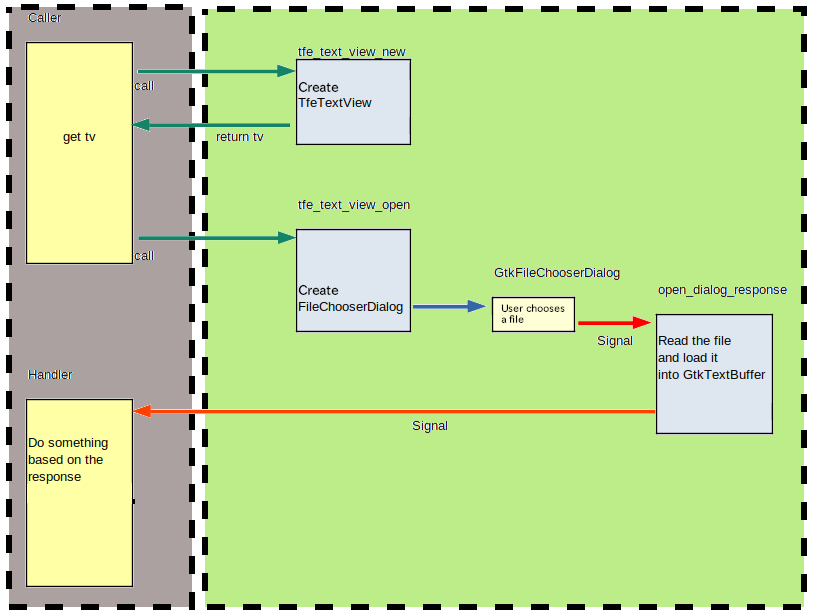
\includegraphics[width=12.405cm,height=9.225cm]{../image/open.png}
\caption{Caller and TfeTextView}
\end{figure}

\begin{enumerate}
\def\labelenumi{\arabic{enumi}.}
\tightlist
\item
  A caller gets a pointer \passthrough{\lstinline!tv!} to a TfeTextView
  instance by calling \passthrough{\lstinline!tfe\_text\_view\_new!}.
\item
  The caller connects the handler (left bottom in the diagram) and the
  signal ``open-response''.
\item
  It calls \passthrough{\lstinline!tfe\_text\_view\_open!} to prompt the
  user to select a file from GtkFileChooserDialog.
\item
  The dialog emits a signal and it invokes the handler
  \passthrough{\lstinline!open\_dialog\_response!}.
\item
  The handler reads the file and inserts the text into GtkTextBuffer and
  emits a signal to inform the status as a response code.
\item
  The handler out of the TfeTextView receives the signal.
\end{enumerate}

\hypertarget{getting-gfile}{%
\subsection{Getting Gfile}\label{getting-gfile}}

\passthrough{\lstinline!gtk\_text\_view\_get\_file!} is a simple
function shown as follows.

\begin{lstlisting}[language=C, numbers=left]
GFile *
tfe_text_view_get_file (TfeTextView *tv) {
  g_return_val_if_fail (TFE_IS_TEXT_VIEW (tv), NULL);

  if (G_IS_FILE (tv->file))
    return g_file_dup (tv->file);
  else
    return NULL;
}
\end{lstlisting}

The important thing is to duplicate \passthrough{\lstinline!tv->file!}.
Otherwise, if the caller frees the GFile object,
\passthrough{\lstinline!tv->file!} is no more guaranteed to point the
GFile. Another reason to use \passthrough{\lstinline!g\_file\_dup!} is
that GFile isn't thread-safe. If you use GFile in the different thread,
the duplication is necessary. See
\href{https://docs.gtk.org/gio/method.File.dup.html}{Gio API Reference,
g\_file\_dup}.

\hypertarget{the-api-document-and-source-file-of-tfetextview.c}{%
\subsection{The API document and source file of
tfetextview.c}\label{the-api-document-and-source-file-of-tfetextview.c}}

Refer API document of TfeTextView in the appendix. Its original markdown
file is under the directory \passthrough{\lstinline!src/tfetextview!}.

All the source files are listed in Section 16. You can find them under
src/tfe5 and src/tfetextview directories.
